\documentclass[11pt]{article}
\usepackage[margin=1in]{geometry}
\usepackage{amsmath}
\usepackage{amssymb}
\usepackage{tikz}
\usepackage{graphicx}
\usetikzlibrary{shapes.geometric, arrows, positioning, shapes}

\tikzstyle{startstop} = [rectangle, rounded corners, minimum width=3cm, minimum height=1cm, text centered, draw=black, fill=red!30]
\tikzstyle{process} = [rectangle, minimum width=3cm, minimum height=1cm, text centered, draw=black, fill=orange!30]
\tikzstyle{decision} = [diamond, minimum width=3cm, minimum height=1cm, text centered, draw=black, fill=green!30]
\tikzstyle{arrow} = [thick,->,>=stealth]

\begin{document}

\title{AAH Code Architecture Notes}
\date{06/07/2025}
\author{Research Notes}
\maketitle

\section{Overview}

OK! Recently we were write code for AAH. The goal of today is to have a rough (DMRG?) of the agreement between fluid and the matched case, as a function of $U_k$ and $V_k$.

The marginal flying to do it a cold material. Reason: So I trying to get a lot more complex terms. We can do this:

\section{Function Architecture}

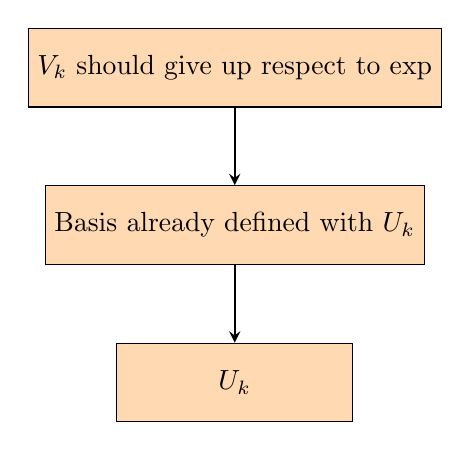
\begin{tikzpicture}[node distance=2cm]
\node (start) [process] {$V_k$ should give up respect to exp};
\node (basis) [process, below of=start] {Basis already defined with $U_k$};
\node (uk) [process, below of=basis] {$U_k$};
\draw [arrow] (start) -- (basis);
\draw [arrow] (basis) -- (uk);
\end{tikzpicture}

\section{Cluster Process Flow}

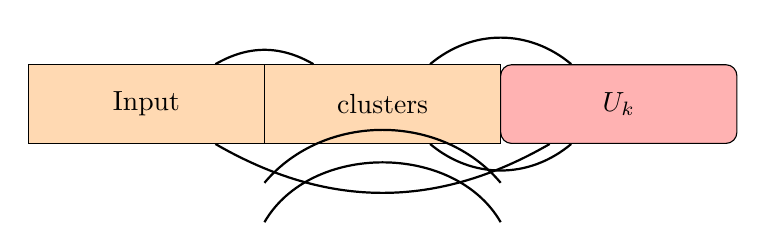
\begin{tikzpicture}[node distance=2.5cm]
% Define nodes - representing the curved diagram from the right side
\node (input) [process] at (0,2) {Input};
\node (cluster) [process] at (3,2) {clusters};
\node (uk) [startstop] at (6,2) {$U_k$};

% Draw the curved flow lines similar to the handwritten diagram
\draw [thick, bend left=30] (input) to (cluster);
\draw [thick, bend right=40] (cluster) to (uk);
\draw [thick, bend left=40] (cluster) to (uk);
\draw [thick, bend right=30] (input) to (uk);

% Add some curved decorative lines to match the handwritten style
\draw [thick, bend left=50] (1.5,1) to (4.5,1);
\draw [thick, bend left=60] (1.5,0.5) to (4.5,0.5);
\end{tikzpicture}

\section{Main Prediction}

I think the main prediction occurs when we get closer to $V_k \to \infty$. There seems to be signal as we go to this.

\section{Additional Notes}

The script has been tested. The iteration technique seems correct - we need to devise signal as we set $V_k$.

\end{document}